\documentclass[12pt]{report}

\usepackage{palatino}
\usepackage{geometry}                % See geometry.pdf to learn the layout options. There are lots.
\geometry{letterpaper}                   % ... or a4paper or a5paper or ...
\usepackage[parfill]{parskip}    % Activate to begin paragraphs with an empty line rather than an indent
\usepackage{graphicx}
\usepackage{amssymb}
\usepackage{epstopdf}
\usepackage{color}
\usepackage{float}
\usepackage{gensymb}
\usepackage{amsmath}
\usepackage{siunitx}
\DeclareGraphicsRule{.tif}{png}{.png}{`convert #1 `dirname #1`/`basename #1 .tif`.png}

\usepackage{fancyhdr}
\usepackage{url}
\usepackage{amsmath}
\usepackage{boxedminipage}
\setlength{\hoffset}{-1in}
\setlength{\voffset}{-1in}
\setlength{\oddsidemargin}{1in}
\setlength{\textwidth}{6.5in}
\setlength{\evensidemargin}{1in}
\setlength{\topmargin}{.75in}
\setlength{\headheight}{.25in}
\setlength{\headsep}{.25in}
\setlength{\topskip}{0in}
\setlength{\footskip}{.5in}
\setlength{\textheight}{9in}
\setlength{\parsep}{72pt}
\setlength{\parindent}{0pt}
\usepackage{hyperref}
\usepackage{natbib}
\usepackage{pdflscape}
\usepackage{rotating}
\usepackage{listings}
\lstset{
  basicstyle=\footnotesize\ttfamily,
  language=matlab}

%\lhead[]{}      % Note the brackets!
%\rhead[]{}
%\lfoot[\thepage]{}
%\rfoot[]{\thepage}
\cfoot{}
% \rhead{$\chi$POD COMPASS SUMMARY}
\lhead{\thepage}

\usepackage[small,normal,bf,up]{caption}
\renewcommand{\captionfont}{\small\itshape}

\setlength{\parskip}{3ex plus 0.5ex minus 0.2ex}
\linespread{1}

\usepackage{sidecap}
\usepackage{float}

% The following makes ODEs and PDEs easier to write.
% For an example, see the second problem below. - Vallis Solution template
\newcommand{\dd}[3][]{{\frac{\dr^{#1} #2}{\dr #3^{#1}}}}
\newcommand{\pp}[3][]{{\frac{\partial^{#1} #2}{\partial #3^{#1}}}}
\newcommand{\DD}[1]{{\frac{\D#1}{\D t}}}
% example: \pp[2]y x

\newcommand\ppx{\pp{}{x}}
\newcommand\ppy{\pp{}{y}}
\newcommand\ppt{\pp{}{t}}


\title{The $\chi$pod and gusT processing package}
\author{Johannes Becherer, Sally Warner, Deepak Cherian}
\date{Last updated: December 11, 2017}

% Definition of \maketitle
\makeatletter
\def\makenewtitle{{
\thispagestyle{plain}
\centering
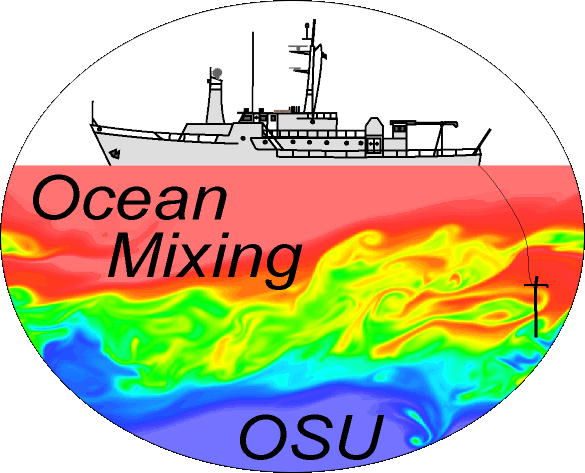
\includegraphics[width=0.4\textwidth]{figs/omg_logo.png} \\[23ex]
\vspace*{\fill}
{\Huge \@title }\\[4ex]
{\large  \@author}\\[4ex]
\@date\\
\vspace*{\fill}}}

\makeatother


\begin{document}

\pagestyle{fancy}

\makenewtitle
\tableofcontents

\part{Calibration}
\chapter{Compass}

It can be confusing how the angles from the compass in $\chi$pods compare to flow direction, and how to ensure correct compass calibration. This document will cover the following:
\begin{enumerate}
\item How the compass is orientated within the $\chi$pod
\item How to convert from $\chi$pod compass angle to flow angle
\item How to include a compass offset
\item How to include magnetic declinations
\item Checking compass calibration with Pitot and ADCP
\item Errors to be aware of
\end{enumerate}

\section{Compass orientation within the $\chi$pod}

If the compass is placed correctly within the $\chi$pod, it will be orientated such that it points towards the sensor tips. Therefore, it will read 0\degree \, when the sensor tips are pointed northward. Figure \ref{fig:cmpveldiag} shows a diagram of how the compass is orientated within the $\chi$pod.

\begin{figure}
  \centering \centering\noindent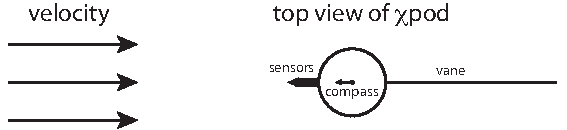
\includegraphics[width=14cm,angle=0]{./figs/compass_and_velocity_diagram.pdf}\\
    \caption{A perfectly installed compass should align with the sensors. The $\chi$pod vane will steer the sensors into the flow.}\label{fig:cmpveldiag}
\end{figure}

\clearpage


\section{Converting from $\chi$pod compass to flow direction}

Converting between compass angle and flow direction is confusing for 2 reasons:

\begin{itemize}
\item The compass uses heading orientation with north = 0\degree, and increasing clockwise such that east = 90\degree, south = 180\degree, and west = 270\degree \,= -90\degree. This is different from velocity for which we typically use vector notation with east = 0\degree, and angles increasing counterclockwise such that north = 90\degree, west = 180\degree, and south = 270\degree \,= -90\degree.
\item Additionally, the sensors point \textit{toward} the flow so they indicate the direction the flow is \textit{coming from} not the direction to which it is going. Therefore, flow to the north would give a compass reading of 180\degree \, since the sensors would be pointed to the south. See Figure \ref{fig:cmpvelangles} for a complete comparison of angles.
\end{itemize}


\begin{figure}[h]
  \centering \centering\noindent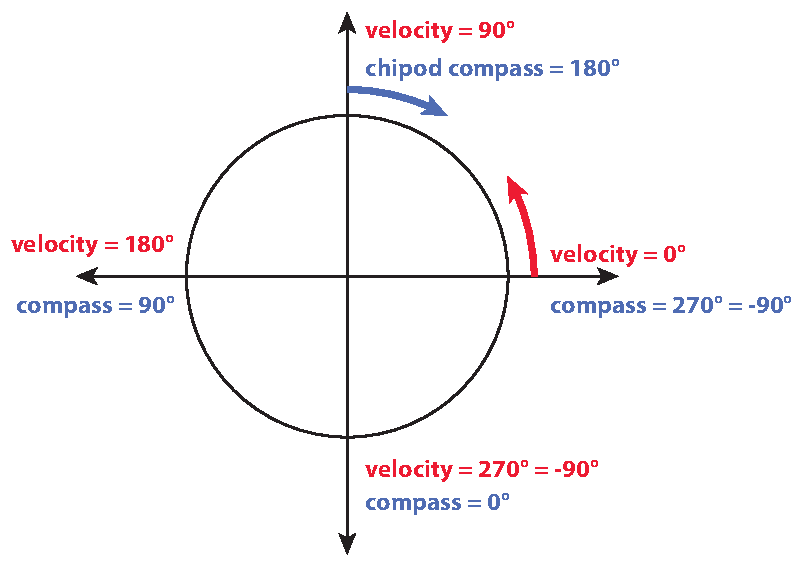
\includegraphics[width=12cm,angle=0]{./figs/compass_and_velocity_angles.pdf}\\
    \caption{Angles of flow direction in vector notation (red) and the corresponding compass readings within the $\chi$pod. This assumes, of course, that the $\chi$pod sensors are vaned to face directly into the flow.}\label{fig:cmpvelangles}
\end{figure}

The formula that can be used to convert $\chi$pod compass angle to flow direction (in vector reference frame) is:
\begin{equation}
\theta_{flow} = -\left(\theta_{compass} + 90\degree\right)
\end{equation}

Alternatively, to convert from flow direction to compass:
\begin{equation}
\theta_{compass} = -\left(\theta_{flow} + 90\degree\right)
\end{equation}

\section{How to find the compass offset}
When the $\chi$pods are built, the compass may not be put into the $\chi$pod casing precisely such that the compass points directly to the sensors. Therefore, the compass is calibrated prior to deployment so we know what the offset is between the sensor direction and the compass direction. To do this, the engineers take the $\chi$pod into the woods away from magnetic sources and point the sensors to the north. They wait a minute, then rotate the $\chi$pod 10\degree \,clockwise. They repeat this all the way around the circle until the $\chi$pod sensors are again pointing toward the north.

Compass calibrations will be saved in a folder called something like ``/Calibrations/compass/'' within each $\chi$pod deployment folder. To view the compass calibrations:

\begin{verbatim}
% load compass calibration file, which would have a name like CMP_00000000.UNT
[data, head] = raw_load_chipod('CMP_00000000.UNT');
figure
plot(data.CMP/10)
\end{verbatim}

This will create a figure that shows the compass calibrations (see Fig. \ref{fig:compasscals} for an example). There should be 37 steps of 10\degree \, increments. Use \texttt{ginput} to select the first and last values to get the offset between the sensor tips and the compass.

\begin{figure}[h]
  \centering \centering\noindent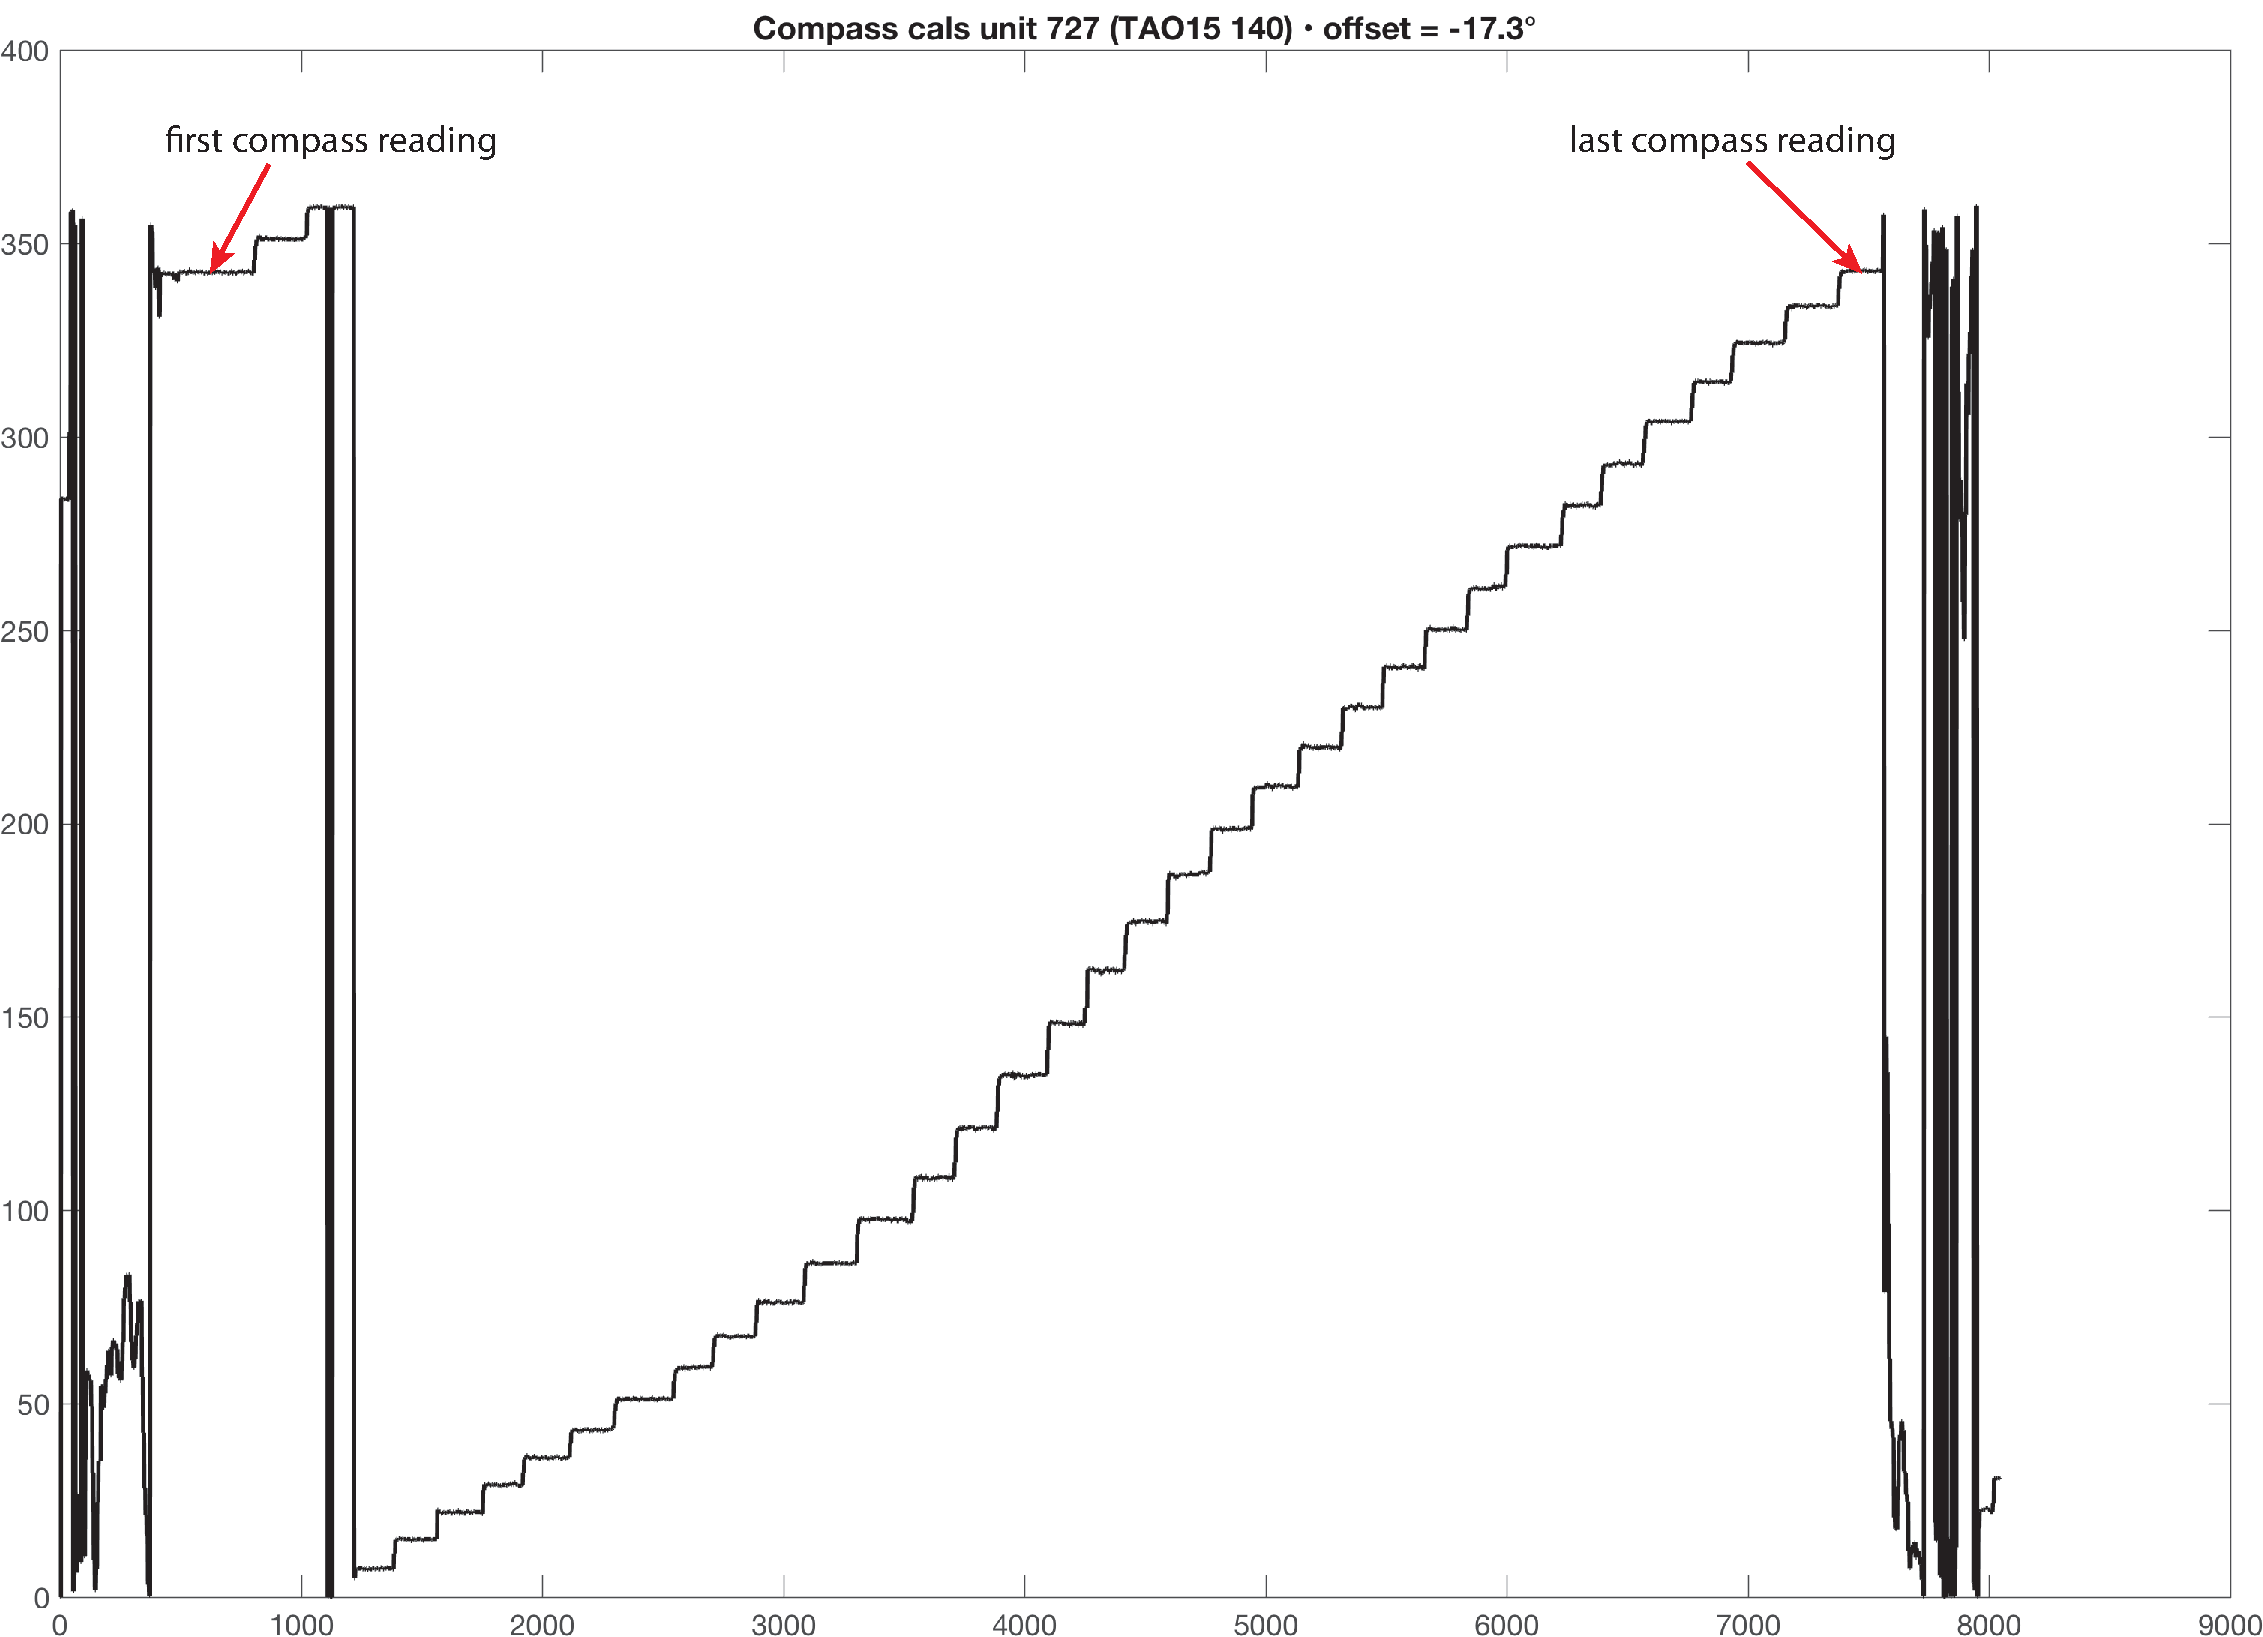
\includegraphics[width=12.5cm,angle=0]{./figs/compass_cals_727.pdf}\\
    \caption{Data from $\chi$pod compass calibration. Compass angle in degrees between 0\degree \, and 360\degree \, on y-axis, unimportant time steps on x-axis. Use \texttt{ginput} to get first and last value. In this case, the offset was found to be 342.7\degree \, = -17.3\degree.}\label{fig:compasscals}
\end{figure}


To apply this offset to the header.mat calibration file, use the following commands in MATLAB. \texttt{UNT} is the unit number, \texttt{DIR} is the directory of the $\chi$pod processing which contains folders like calib, mfiles, input, proc, raw, etc., and \texttt{OFFSET} is the angle found using ginput from the compass calibration file. It is important to include the negative offset in the header file (head.mat) because this is the value that is \textit{added} to all of the compass readings.

\begin{verbatim}
% move to the correct directory
    cd DIR
% load the header file that includes all of the calibrations
    load calib/header.mat
% display the compass calibration which should be [0; 1; 0; 0; 0]
    head.coef.CMP
% add the offset to the header. **Input the NEGATIVE of OFFSET**
    head.coef.CMP(1) = -OFFSET
% save the updated header
    save calib/header.mat head
\end{verbatim}



\section{How to include magnetic declinations}

Magnetic declination arises because the magnetic field of the earth is not uniform. This is especially important in the Pacific Northwest: a compass pointing directly north will give a reading of about 15\degree \, east of north due to the large mass of the Cascade mountains to the east. Note that the magnetic declination changes slowly over time. This needs to be included in the compass calibrations!

Look up the magnetic declinations in Corvallis where the instrument was calibrated and at the deployment location on the following website:
\begin{verbatim}
https://www.ngdc.noaa.gov/geomag-web/#declination
\end{verbatim}
In 2017, the magnetic declination in Corvallis was about 15\degree E (Fig. \ref{fig:declination}). The magnetic declination at 0\degree, 140\degree W, where many $\chi$pods are deployed is 9.3\degree.

\begin{figure}
  \centering \centering\noindent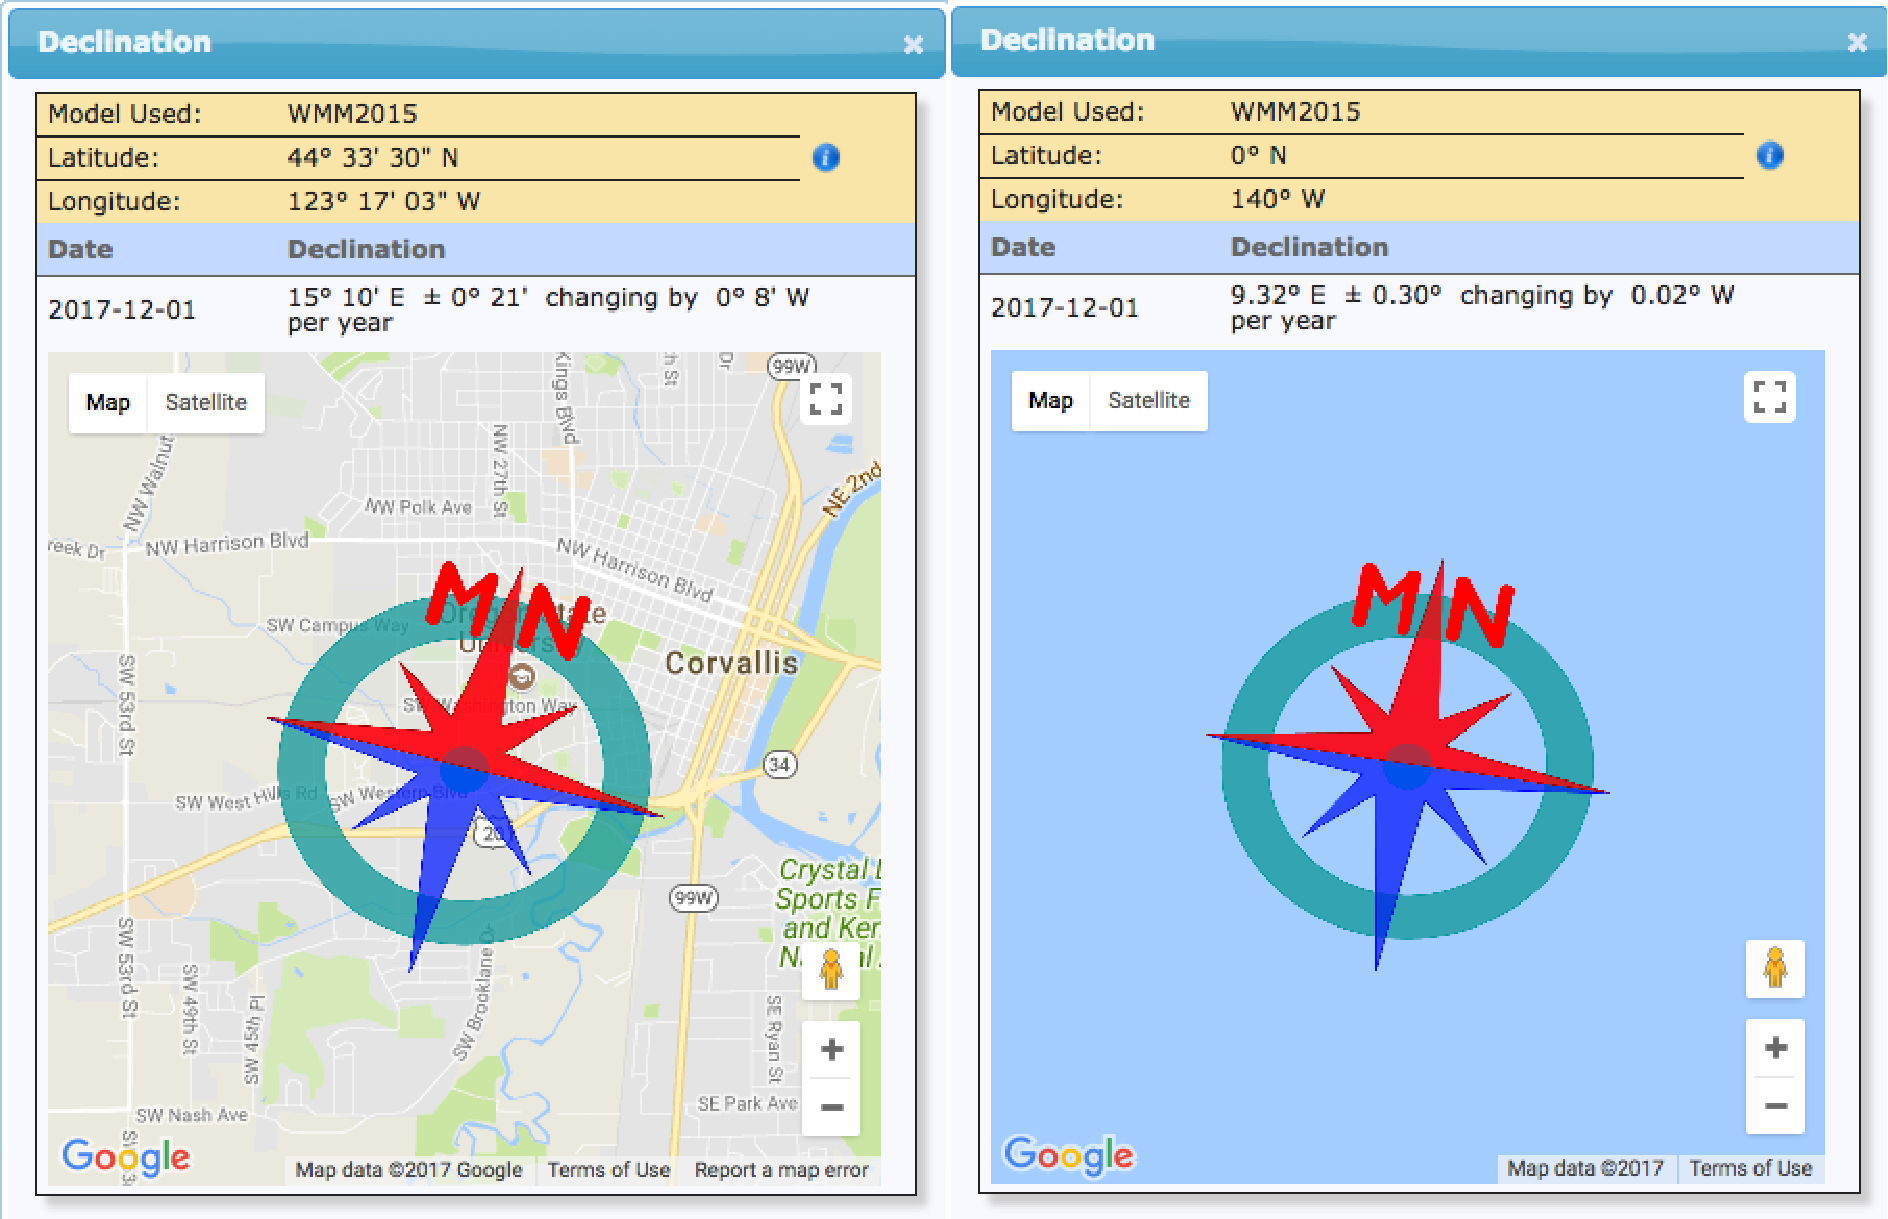
\includegraphics[width=14cm,angle=0]{./figs/declination_both.pdf}\\
    \caption{The magnetic declination in Corvallis and at 0\degree, 140\degree W on December 1, 2017.}\label{fig:declination}
\end{figure}

Now, instead of just inputting the OFFSET into the header calibrations, you'll want to include the declinations. Repeat the steps in the previous section, but include the declinations:
\begin{verbatim}
% add the offset and declinations to the header
    head.coef.CMP(1) = -OFFSET - DECL_CORVALLIS + DECL_DEPLOYMENT
% don't forget to save the updated header
    save calib/header.mat head
\end{verbatim}

For our example, the offset was -17.3\degree, the magnetic declination in Corvallis was 15.2\degree, and the magnetic declination at the deployment location was 9.3\degree. Therefore, we set the header coefficient to be 11.4\degree \, ($--17.3 - 15.2 + 9.3 = 11.4$).

Alternately, within the $\chi$pod\_gust software, you can include the compass offset and magnetic declinations in \texttt{pre\_driver.m} (shown with example values input into code):
\begin{verbatim}
LINE 24      modify_header = 1;   % if 1, specify header corrections below
LINE 25                           % (e.g. declination)
LINE 26
LINE 27      % get declination: https://www.ngdc.noaa.gov/geomag-web/#declination
LINE 28      CompassOffset = -17.3; % exact value from calibration file
LINE 29                           % (no sign changes!)
LINE 30      DeployDecl = 9.3; % at deployment location
LINE 31      CorvallisDecl = 15+10/60; % at corvallis
...
LINE 81      head.coef.CMP(1) = -CompassOffset - CorvallisDecl + DeployDecl;
\end{verbatim}

\clearpage
\section{Checking compass calibrations with Pitot and ADCP}

If you have ADCP data and the compass has been calibrated correctly, pitot derived velocities should match up very well with ADCP velocities. Fig. \ref{fig:pitotADCP} shows the output from \texttt{calibrate\_pitot}. Additonally, when \texttt{calibrate\_pitot} is run, an angle offset between the ADCP and pitot is printed to the screen. This should be small (i.e. $<5$\degree).

\begin{figure}[h]
  \centering \centering\noindent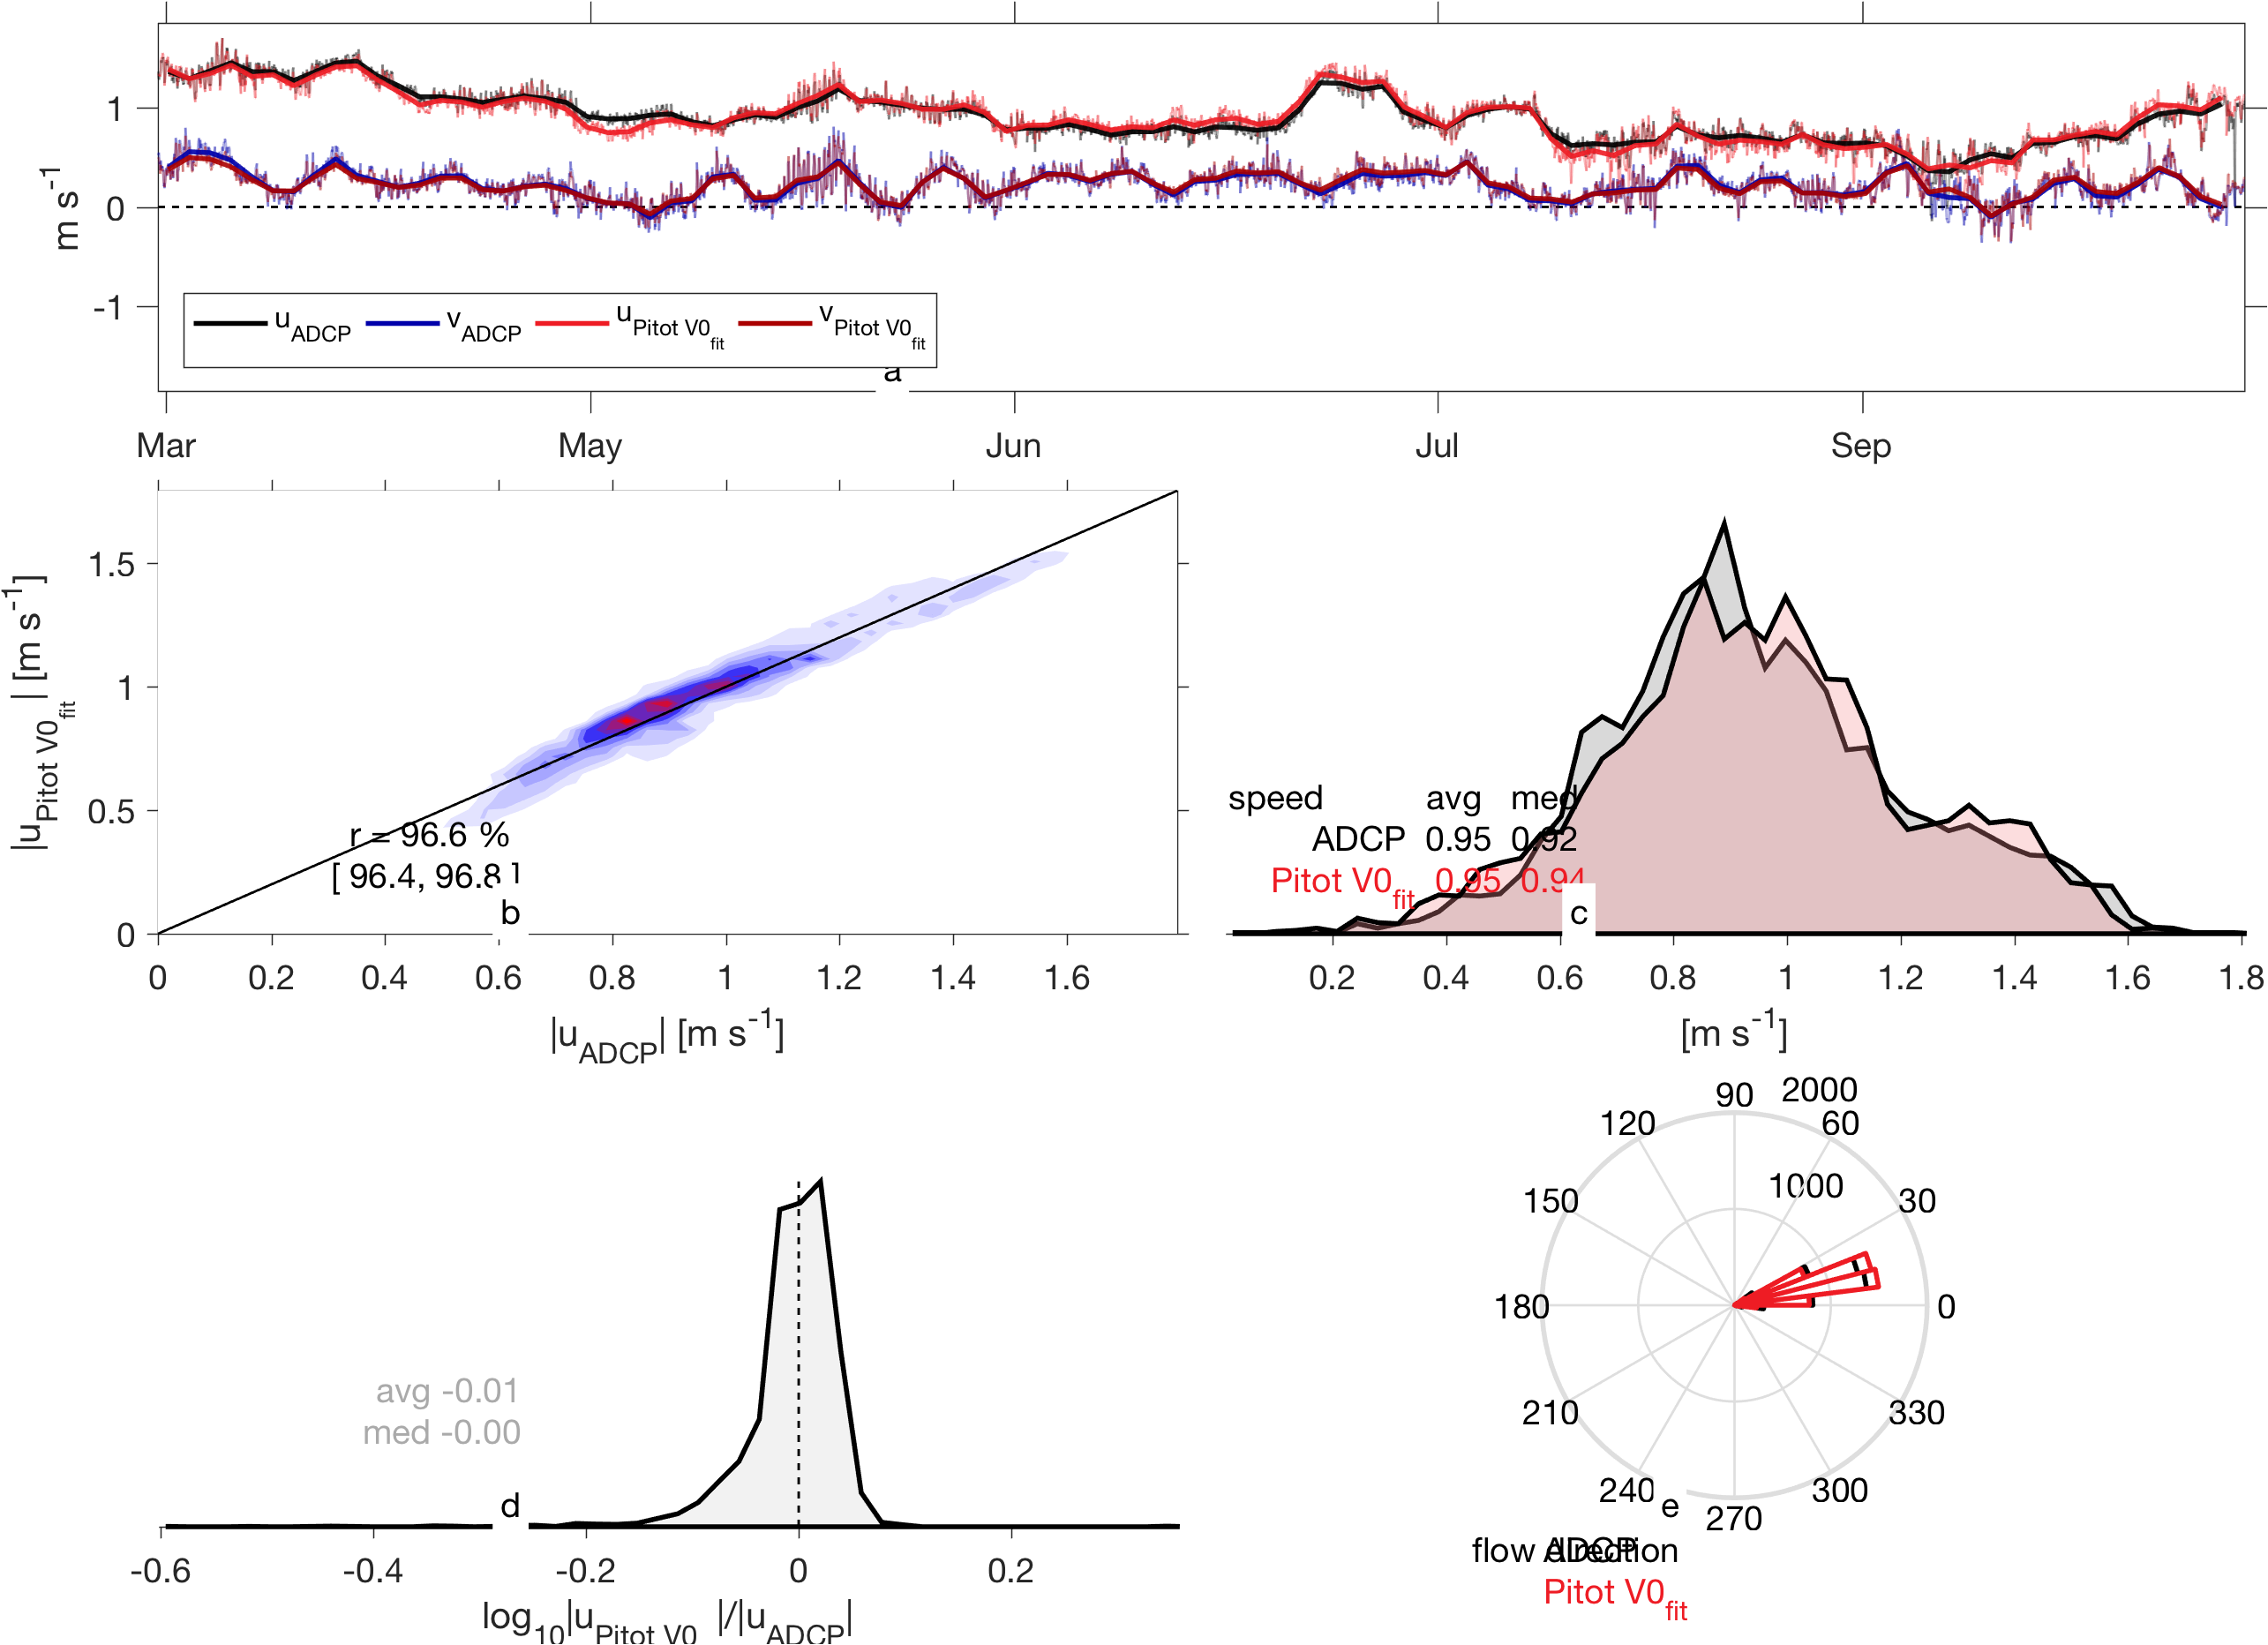
\includegraphics[width=14cm,angle=0]{./figs/Pitot_vs_ADCP_resized.png}\\
    \caption{Output of \texttt{calibrate\_pitot} when the compass has been correctly calibrated. ADCP and pitot velocities match closely.}\label{fig:pitotADCP}
\end{figure}

\section{Errors to be aware of}

There are a few problems that can arise.

\subsection{Nonlinear compass calibrations}
There have been a few cases where the compass calibrations look very nonlinear (e.g. Fig. \ref{fig:badcals}). In other words, the compass steps during the calibration are not all 10\degree. Some are as big as 50\degree, and many are $<5$\degree.

To fix this, we did not use the compass calibration from Fig. \ref{fig:badcals}, which was 195.6\degree. Instead, we manually found the offset that got the compass direction to match the flow direction as measured by the ADCP (Fig. \ref{fig:findcompassoffset}). The new offset is found to be 91.4\degree. A big difference! This would not work as well in cases where the current was not uniformly flowing in one direction as it was for this $\chi$pod.

\begin{figure}[h]
  \centering \centering\noindent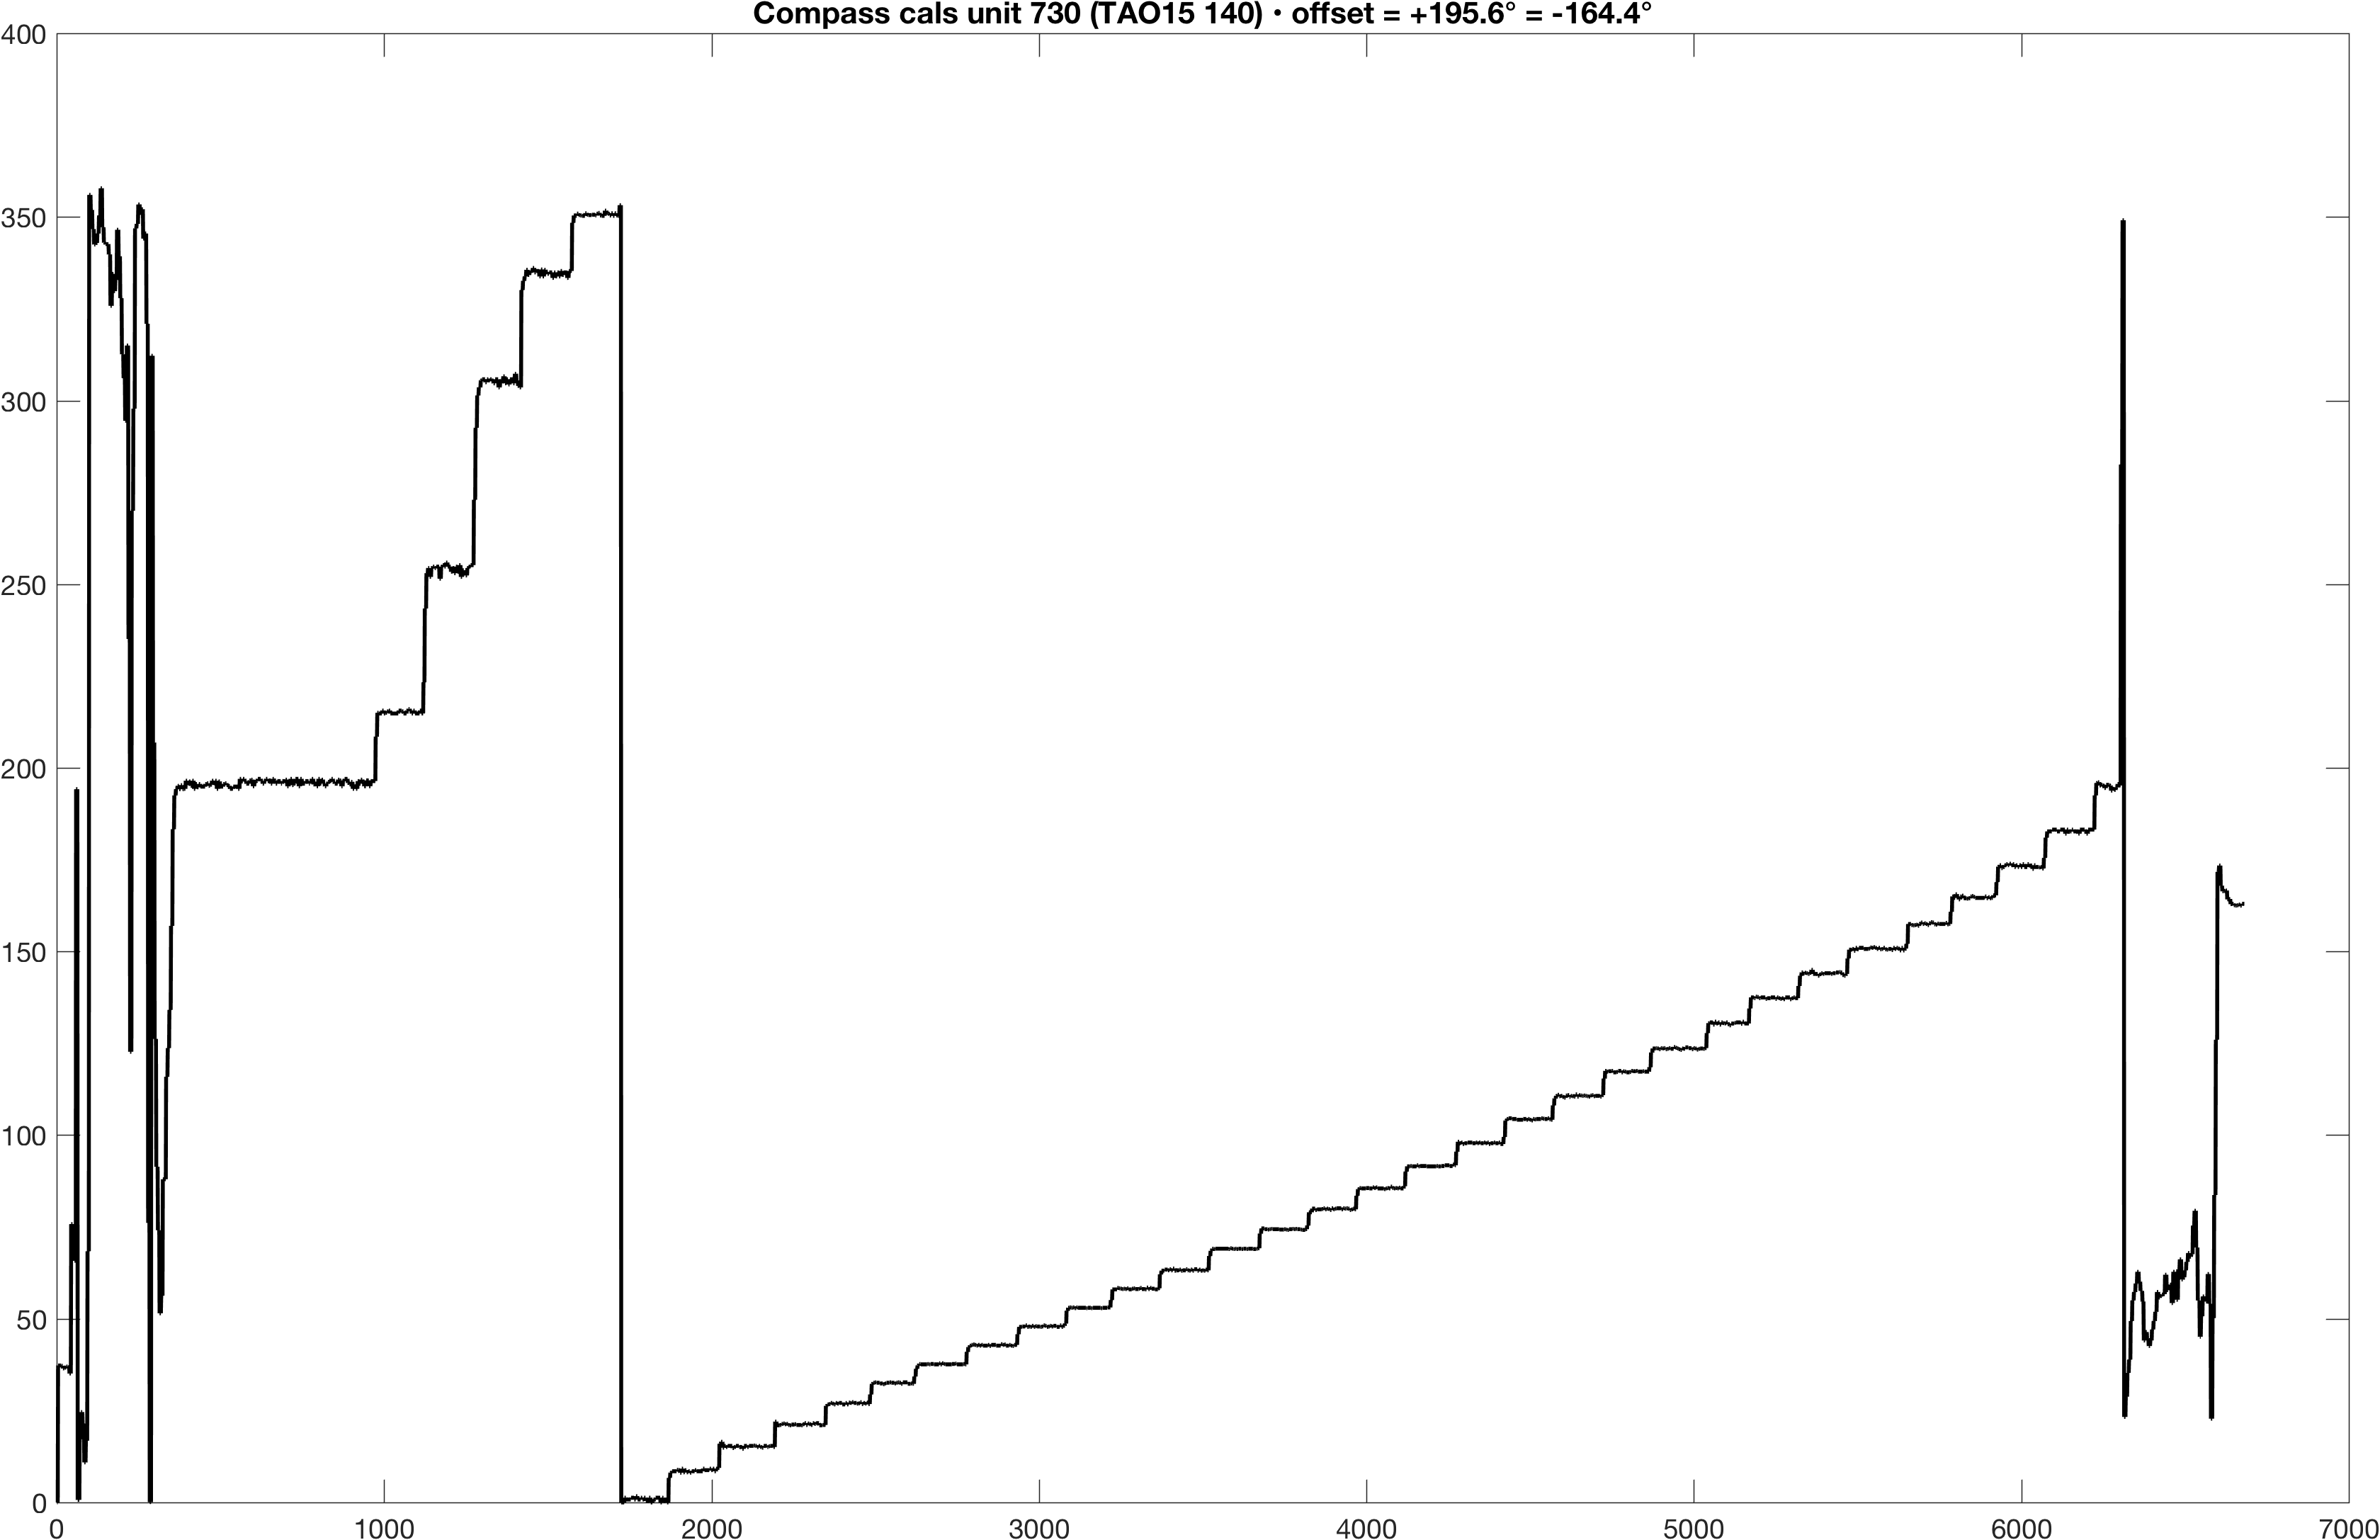
\includegraphics[width=12.5cm,angle=0]{./figs/compass_cals_730.png}\\
    \caption{Example of bad compass calibrations. Not all steps are equal.}\label{fig:badcals}
\end{figure}

\begin{figure}[h]
  \centering \centering\noindent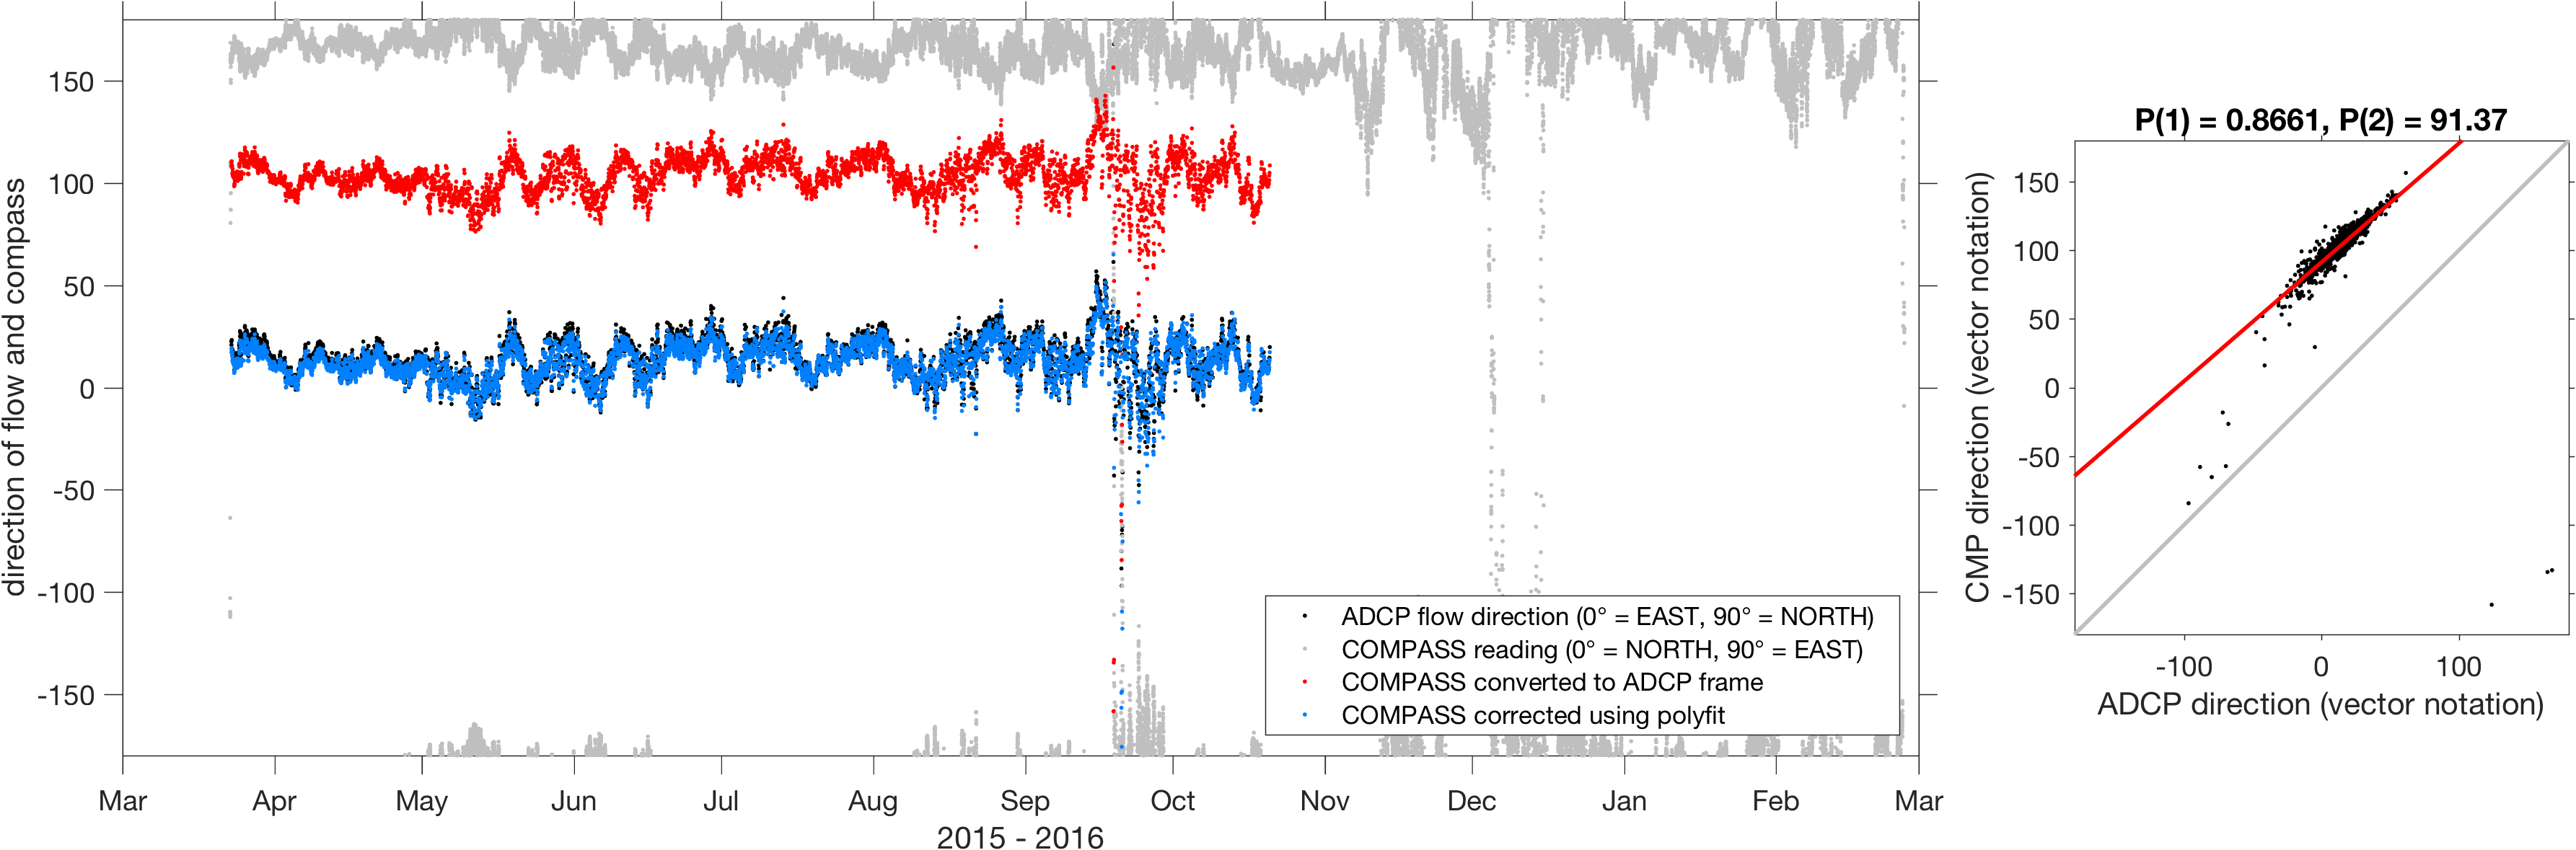
\includegraphics[width=16cm,angle=0]{./figs/compare_ADCP_direction_to_compass.png}\\
    \caption{Manually finding the compass offset that makes the compass match the ADCP. Flow direction from ADCP (black dots), compass readings in heading coordinates (gray dots), compass readings converted to vector coordinates (red), compass readings in vector coordinates with an offset of 91.37\degree \, applied.}\label{fig:findcompassoffset}
\end{figure}

\subsection{Bad comparison between ADCP and Pitot}
Sometimes, the comparison between the ADCP and the pitot are just plain bad. This is somewhat hard to diagnose. Maybe the pitot goes bad. Try doing the calibration over a shorter period of time and look for jumps in the signal. Maybe the compass calibrations are bad, in which case trust the angle given in the ADCP vs pitot comparison.

You can ignore the compass in the $\chi$pod processing by setting
\begin{verbatim}
pflag.master.use_compass = 0;
\end{verbatim}
in \texttt{main\_driver.m}. This will assume that the $\chi$pod is always perfectly vaned directly into the flow. When the compass is bad, the pitot will be able to give speed but not direction unless there is an ADCP to compare to.

\subsection{Declinations already included in the calibration}

There were some cases where the magnetic declination was being included in the compass calibrations. I'm not sure how this was being done. It's impossible to know whether they were or weren't included unless a note is added in the calibration folder. If you suspect this may be the case, (1) ask Pavan if he remembers how the compass was calibrated, (2) try adding and subtracting the declination in Corvallis to see if that helps, or just (3) use the ADCP to pitot comparisons to get the compass offset.

%%% Local Variables:
%%% mode: latex
%%% TeX-master: "docs"
%%% End:

\chapter{Pitot-static tubes}

%%% Local Variables:
%%% mode: latex
%%% TeX-master: "docs"
%%% End:


\part{Processing}
\chapter{\texttt{pre\_driver}}
%%% Local Variables:
%%% mode: latex
%%% TeX-master: "docs"
%%% End:

\chapter{\texttt{main\_driver}}

%%% Local Variables:
%%% mode: latex
%%% TeX-master: "docs"
%%% End:

\chapter{\texttt{combine\_turbulence}}

This is the final step.

\section{Masking criteria/thresholds}
\label{sec:orgccff08d}
\subsection{Background stratification: \texttt{min\_dTdz, min\_N2, additional\_mask\_dTdz}}

Minimum $dT/dz$, $N^2$ required for valid computation of $\chi, K_T, J_q^t$

The Seabird SBE-37 datasheet says (\url{http://www.seabird.com/sbe37si-microcat-ctd})
\begin{itemize}
\item T is accurate to \SI{2e-3}{\celsius}
\item conductivity is accurate to \SI{3e-3}{psu} (approx!)
\end{itemize}

i.e.,
\begin{itemize}
\item dT/dz is accurate to (2x2e-3)/dz
\item dS/dz is accurate to (2x3e-3)/dz
\end{itemize}

\subsection{Sensor deaths: \texttt{T1death, T2death; nantimes\{1,2,3\}}}

\subsection{Averaging: \texttt{avgwindow, avgvalid}}

\subsection{Orientation / sensed-volume-flushing}
\subsection{Background flow speed: \texttt{min\_inst\_spd, min\_spd, additional\_mask\_spd}}

\subsection{Maximum thresholds on $\epsilon, \chi, K_T, J_q^t$}

\subsection{Deglitching: \texttt{deglitch\_window, deglitch\_nstd
}}

\section{Useful Functions}
\subsection{ChooseEstimates}
\subsection{chiold (variable)}
combine\_turbulence saves the \emph{unmasked} chi structure as chiold after calculating Kt, Jqt but before doing any processing. Useful in checking masking.

\subsection{TestMask}
Lets you quickly iterate through various thresholds for a particular criterion.

Throws up a figure with histograms of counts to compare.

Example usage:
\begin{lstlisting}
TestMask(chi, abs(chi.dTdz), '<', [1e-4, 3e-4, 1e-3], 'Tz');\\
\end{lstlisting}

This will iterate and mask using chi.dTdz < 1e-4, then chi.dTdz < 3e-4 and finally chi.dTdz < 1e-3. Each iteration is \textbf{independent} of the previous one.

\subsection{DebugPlots}
Usually, you want to see the effect of different masking thresholds in a small subset of the time series of χ, ε etc.

Example usage:
\begin{lstlisting}
chi = chiold; \% reset to unmasked structure\\
\% apply 3 different thresholds\\
chi1 = ApplyMask(chi, abs(chi.dTdz), '<', 1e-4, 'T\(_{\text{z}}\) < 1e-4');\\
chi2 = ApplyMask(chi, abs(chi.dTdz), '<', 1e-3, 'T\(_{\text{z}}\) < 1e-3');\\
chi3 = ApplyMask(chi, abs(chi.dTdz), '<', 2e-3, 'T\(_{\text{z}}\) < 2e-3');\\
\vspace*{1em}
t0 = datetime(2016, 12, 10);\\
t1 = datenum(2016, 12, 12);\\
tavg = 600;\\
\vspace*{1em}
hf = figure;\\
\% plot 10 minute averages (tavg) of quantities in structure chi\\
\% between [t0, t1] and label them as 'raw' in figure window hf\\
DebugPlots(hf, t0, t1, chi, 'raw', tavg);\\
\vspace*{1em}
\% compare different masking; label appropriately\\
DebugPlots(hf, t0, t1, chi1, '1e-4', tavg);\\
DebugPlots(hf, t0, t1, chi2, '1e-3', tavg);\\
DebugPlots(hf, t0, t1, chi3, '2e-3', tavg);\\
\end{lstlisting}

\subsection{DebugRawData}
The idea is to connect Turb.() to the raw-ish data.

Requires structure T from temp.mat.

\subsection{Histograms2D}

%%% Local Variables:
%%% mode: latex
%%% TeX-master: "docs"
%%% End:



\appendix
\part{Appendix}
\chapter{Using the CEOAS MATLAB servers}

\section{SSH configuration}

\section{Usage}

1. login in  to maltab server
   1) open terminal
   2) type: mats

2. logout
   type twice: exit

3. open matlab on server
   type: mat
   or  : matno    \#(for no display)

4. How to copy from ganges to server-ganges
	cd ~/ganges/
	sh pullFromGanges data/(dir you want to copy)/
        otherwise use scp

%%% Local Variables:
%%% mode: latex
%%% TeX-master: "docs"
%%% End:

\chapter{Useful references}


%%% Local Variables:
%%% mode: latex
%%% TeX-master: "docs"
%%% End:

\chapter{git commands and workflows}
%%% Local Variables:
%%% mode: latex
%%% TeX-master: "docs"
%%% End:

\chapter{Sensor orientations}

\section{$\chi$pod}

\section{Pitot}

from \cite{Moum2015}

{
  \centering
  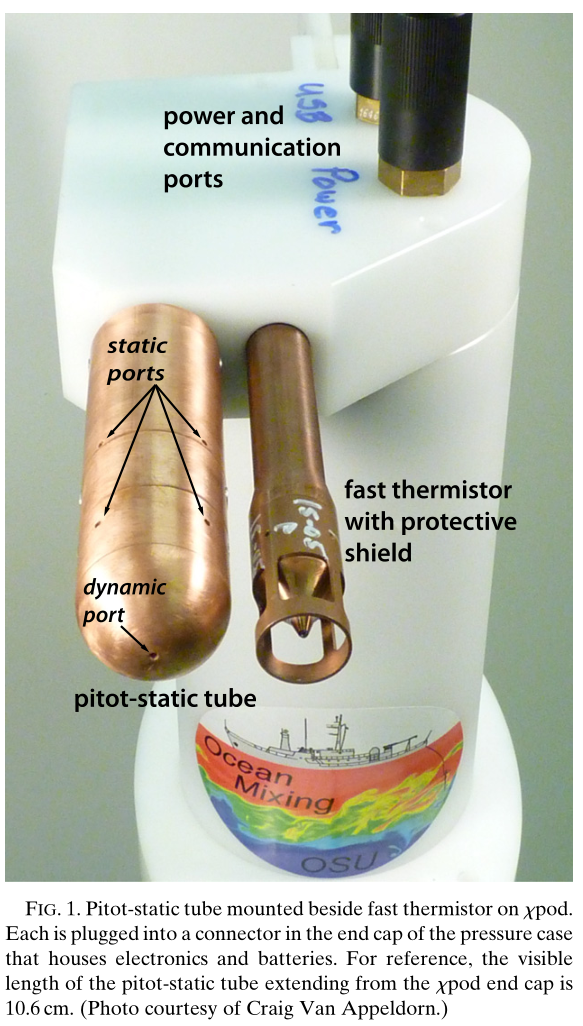
\includegraphics[height=0.9\textheight]{figs/pitot-exterior-chipod.png}
}

{\centering
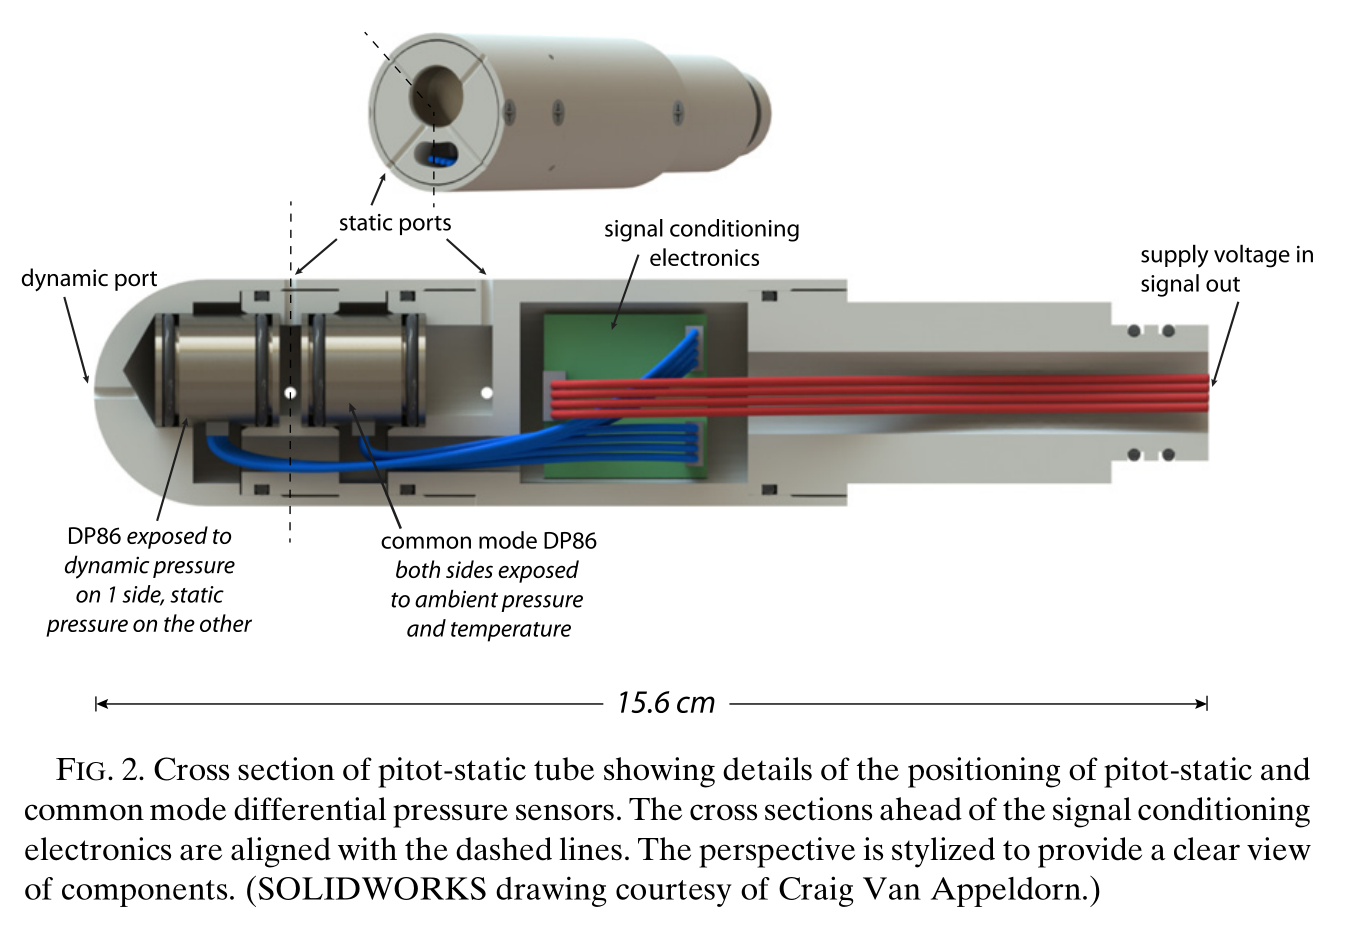
\includegraphics[width=\textwidth]{figs/pitot-cross-section.png}
}
\section{gusT}

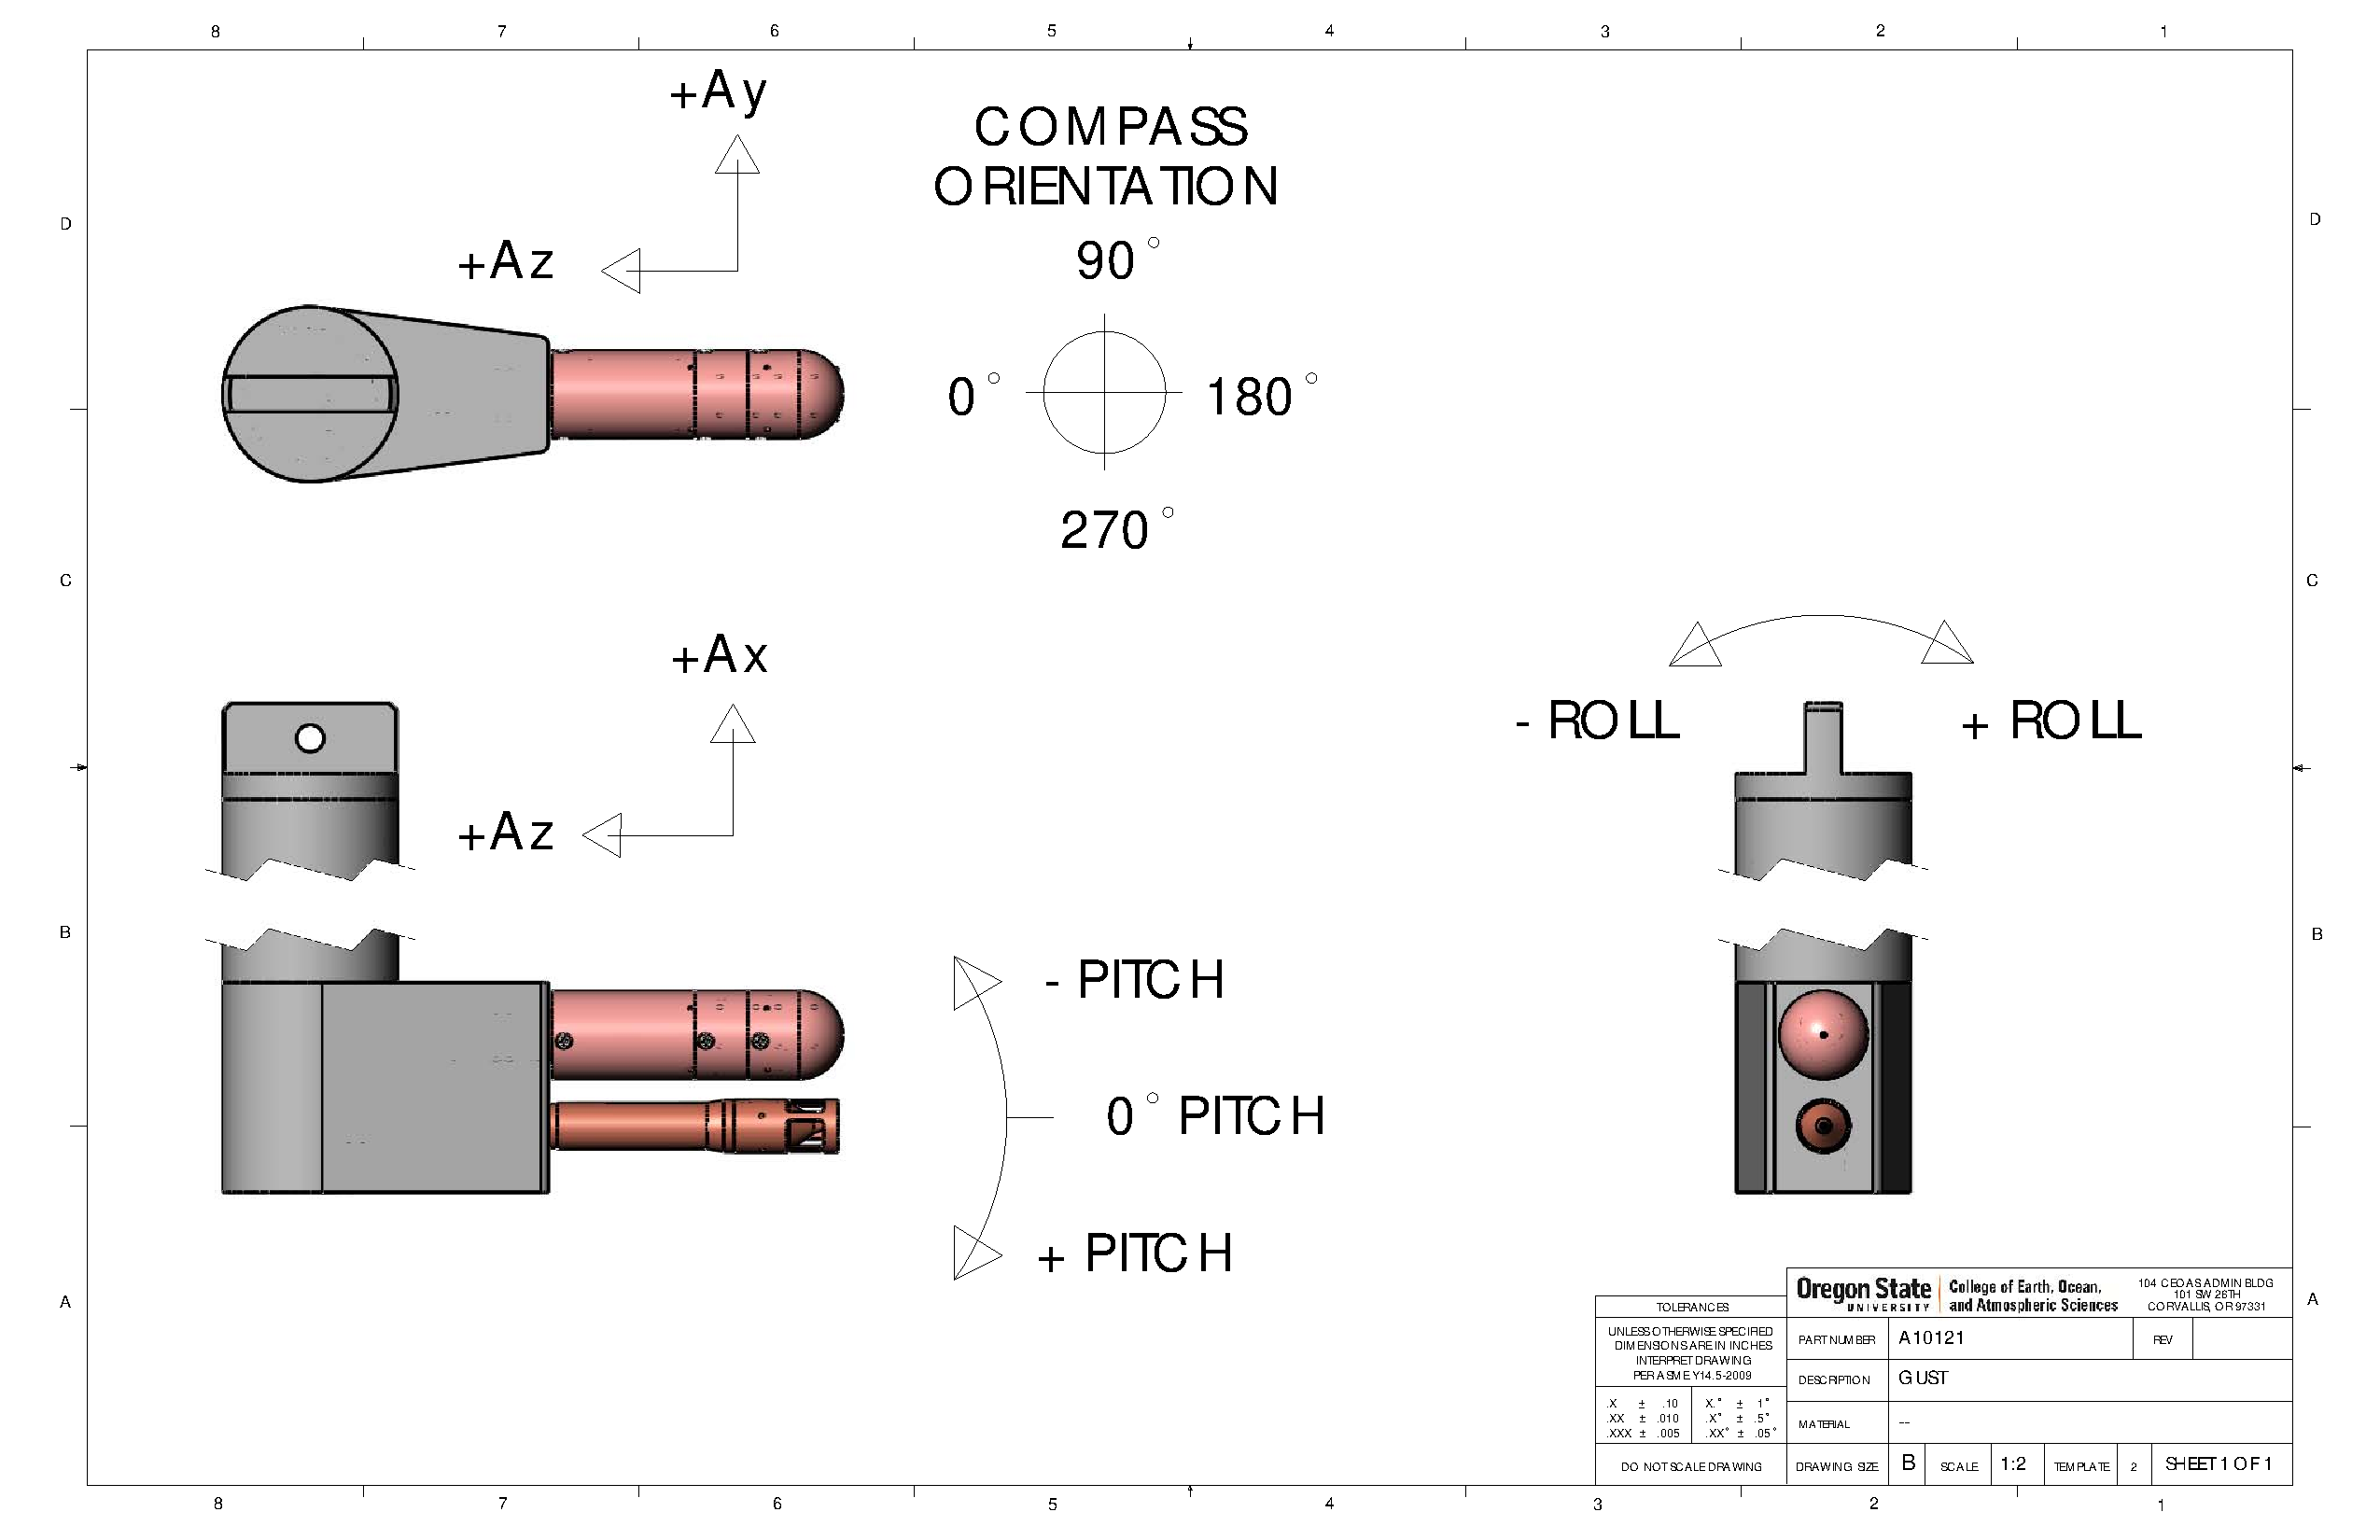
\includegraphics[width=\textwidth]{figs/gooseneck-gust-sensor-orienatation.pdf}

\section{Multi gusT}

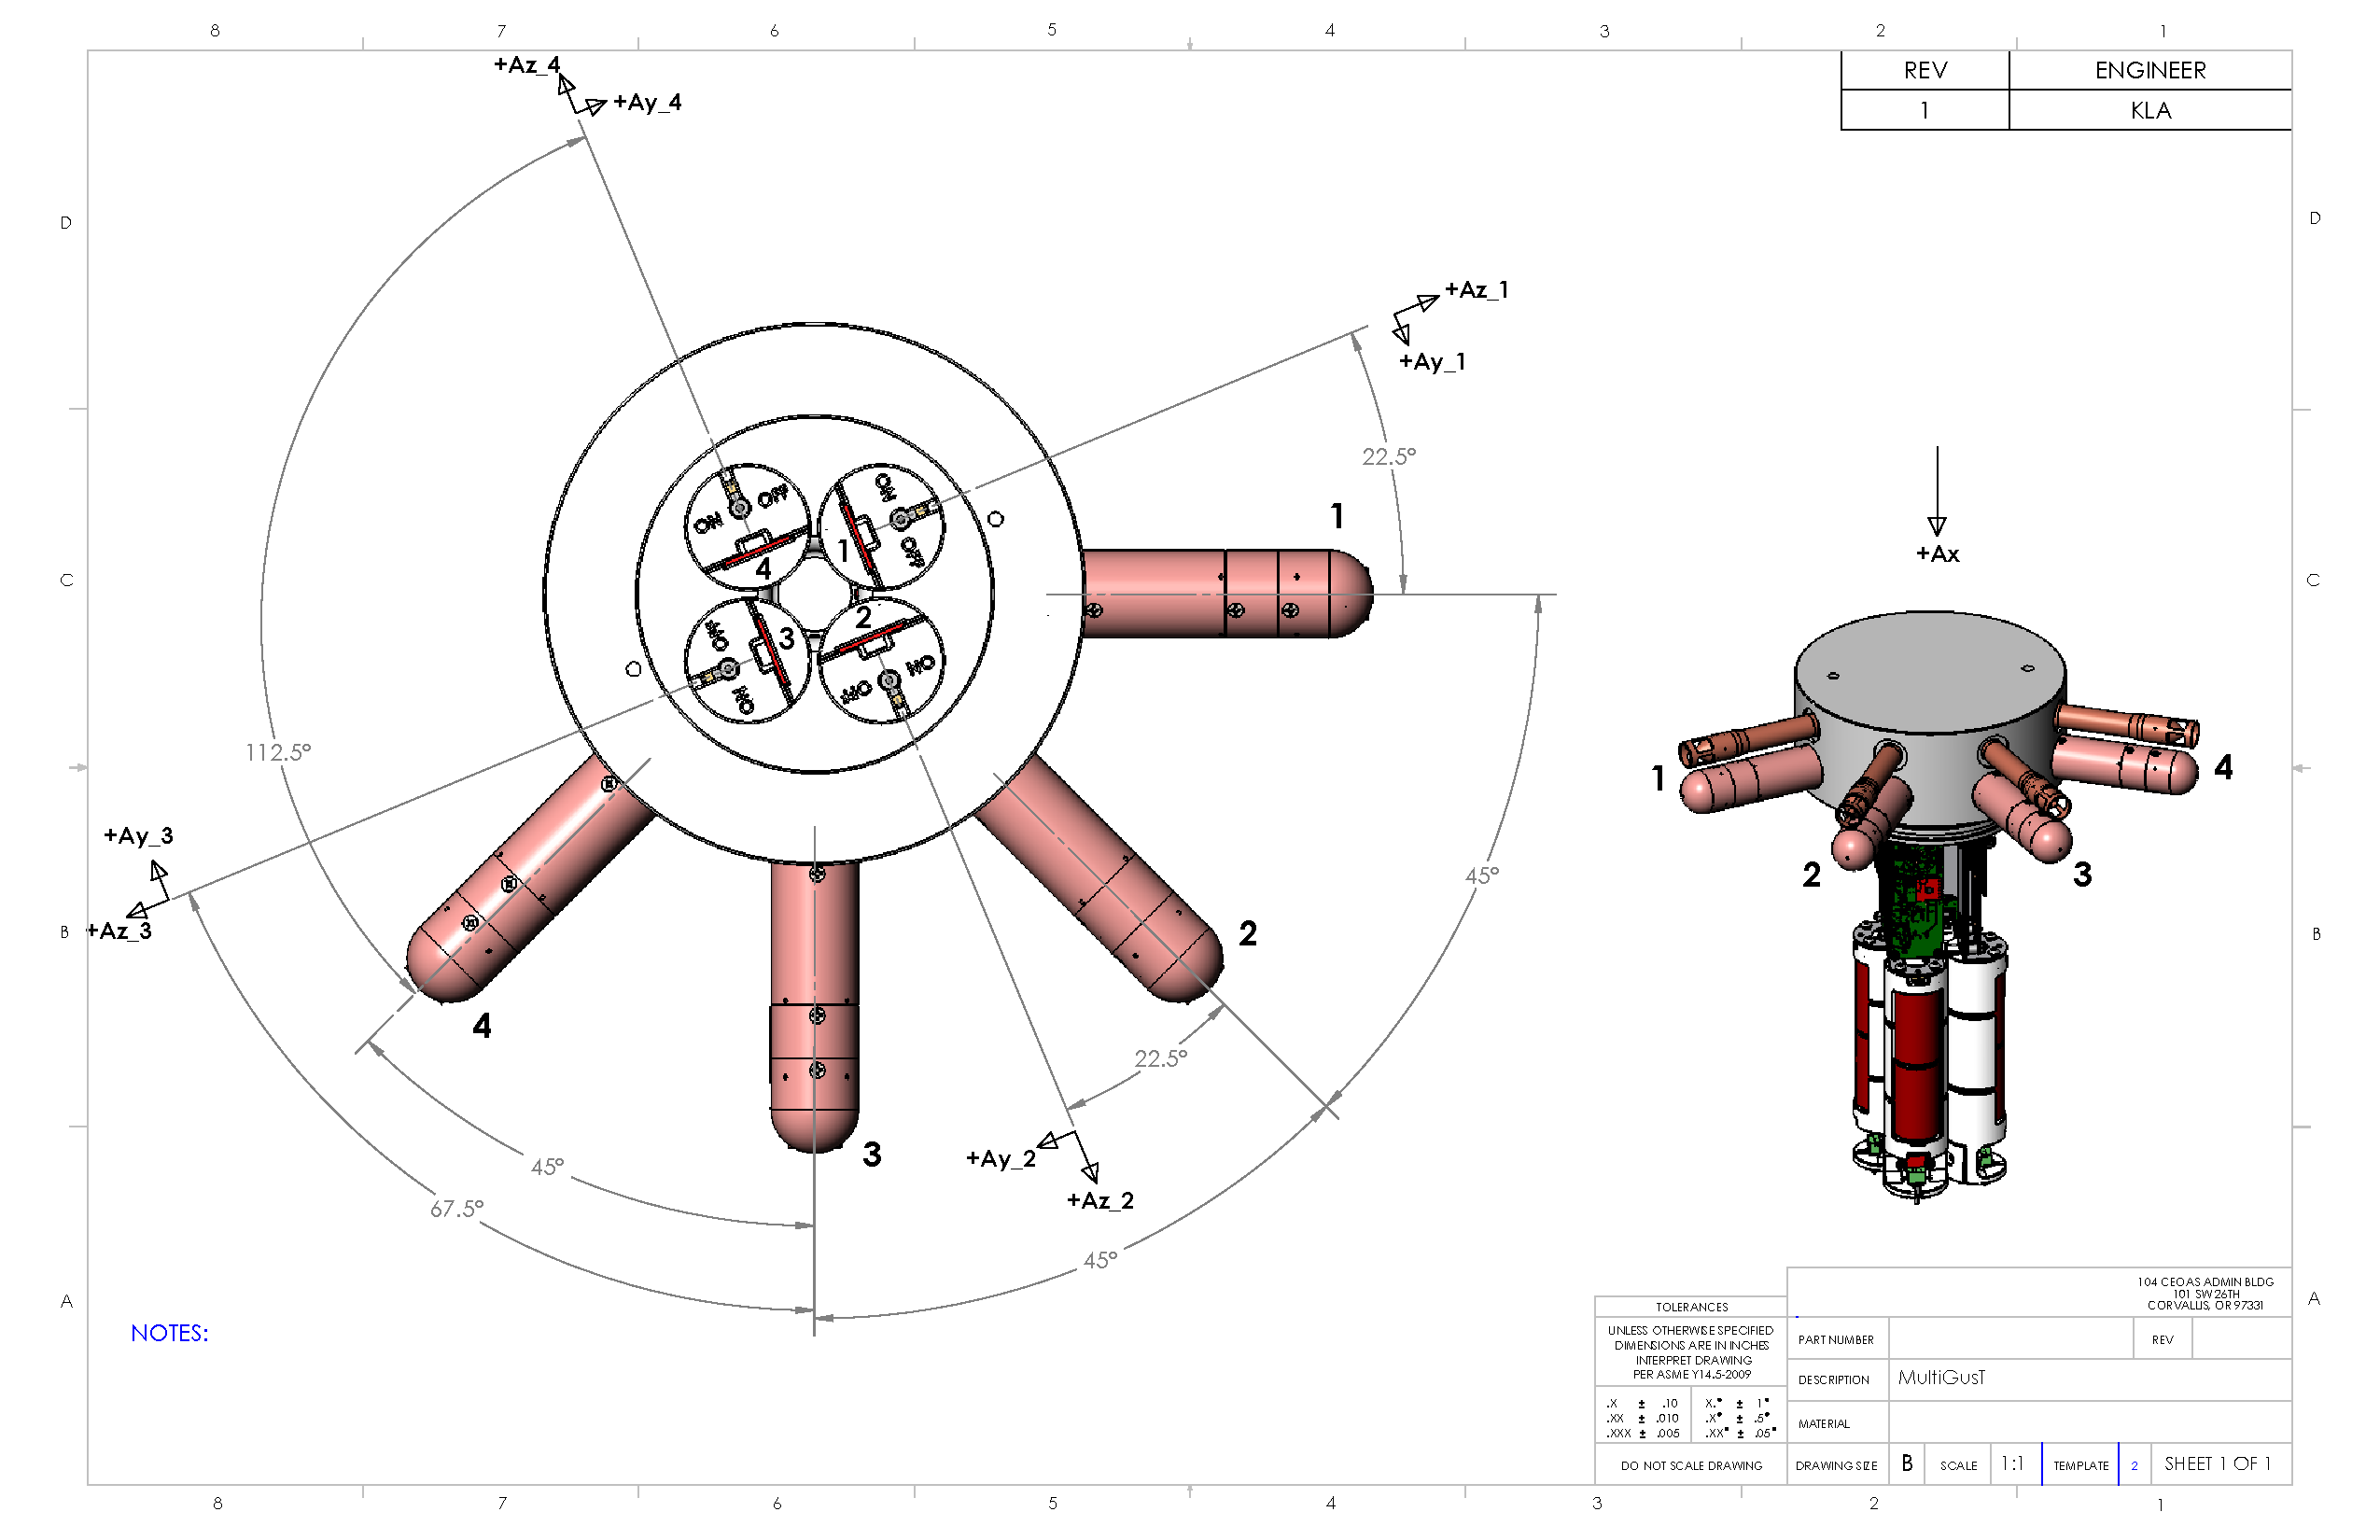
\includegraphics[width=\textwidth]{figs/multigust-sensor-orientation.pdf}
%%% Local Variables:
%%% mode: latex
%%% TeX-master: "docs"
%%% End:


\end{document}
